\subsection{Handwritten records of the experiment}
%    \includegraphics[width=\linewidth]{record/}
\clearpage
\subsection{Additional figures}
\begin{figure}
    \begin{subfigure}[b]{\picwidth}
        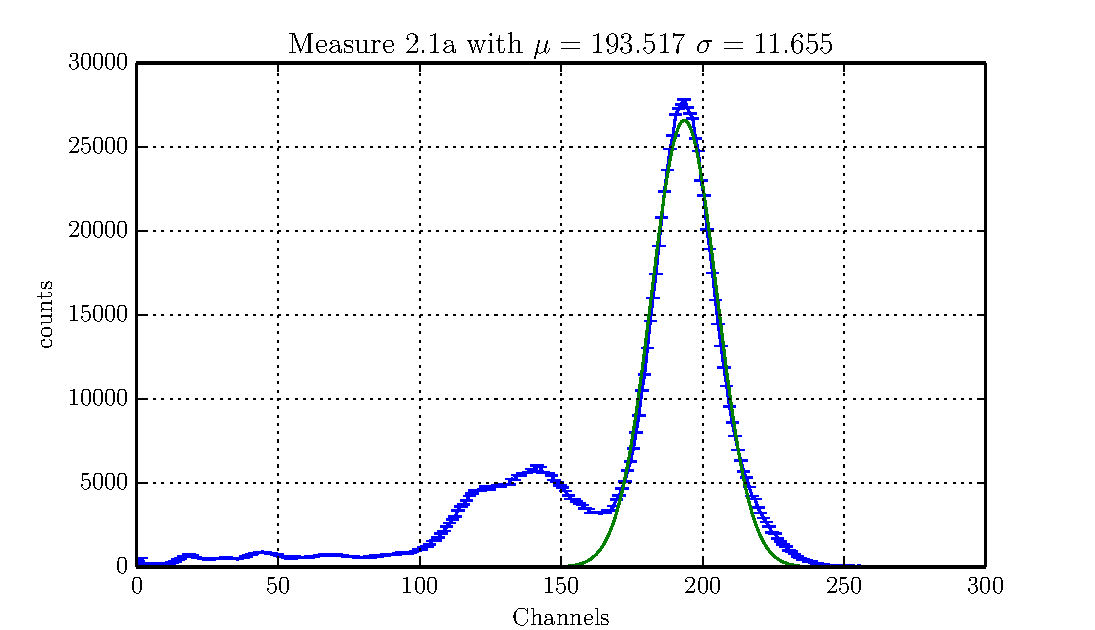
\includegraphics[width=\textwidth]{analysis/figures/plot2_1a}
        \caption{}
    \end{subfigure}\qquad
    \begin{subfigure}[b]{\picwidth}
        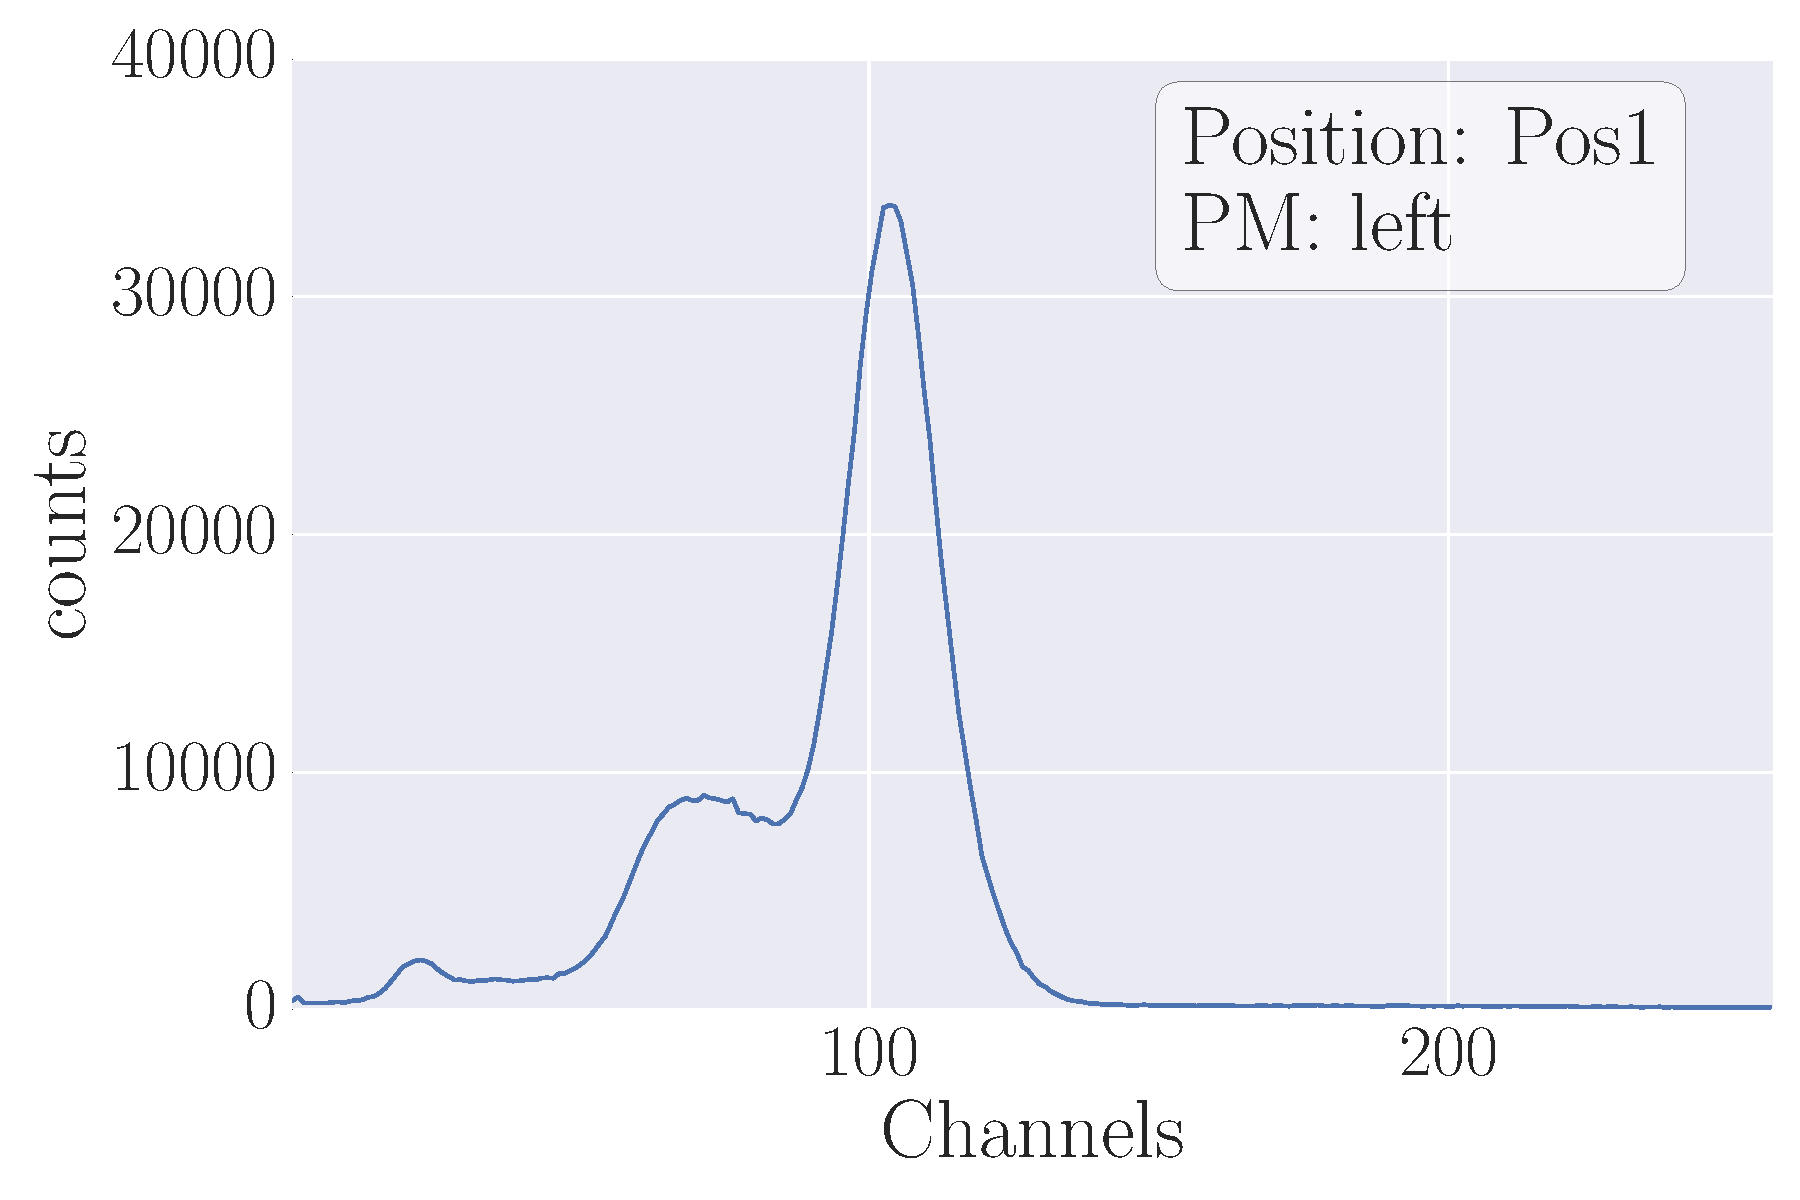
\includegraphics[width=\textwidth]{analysis/figures/plot2_1b}
        \caption{}
    \end{subfigure}
    \begin{subfigure}[b]{\picwidth}
        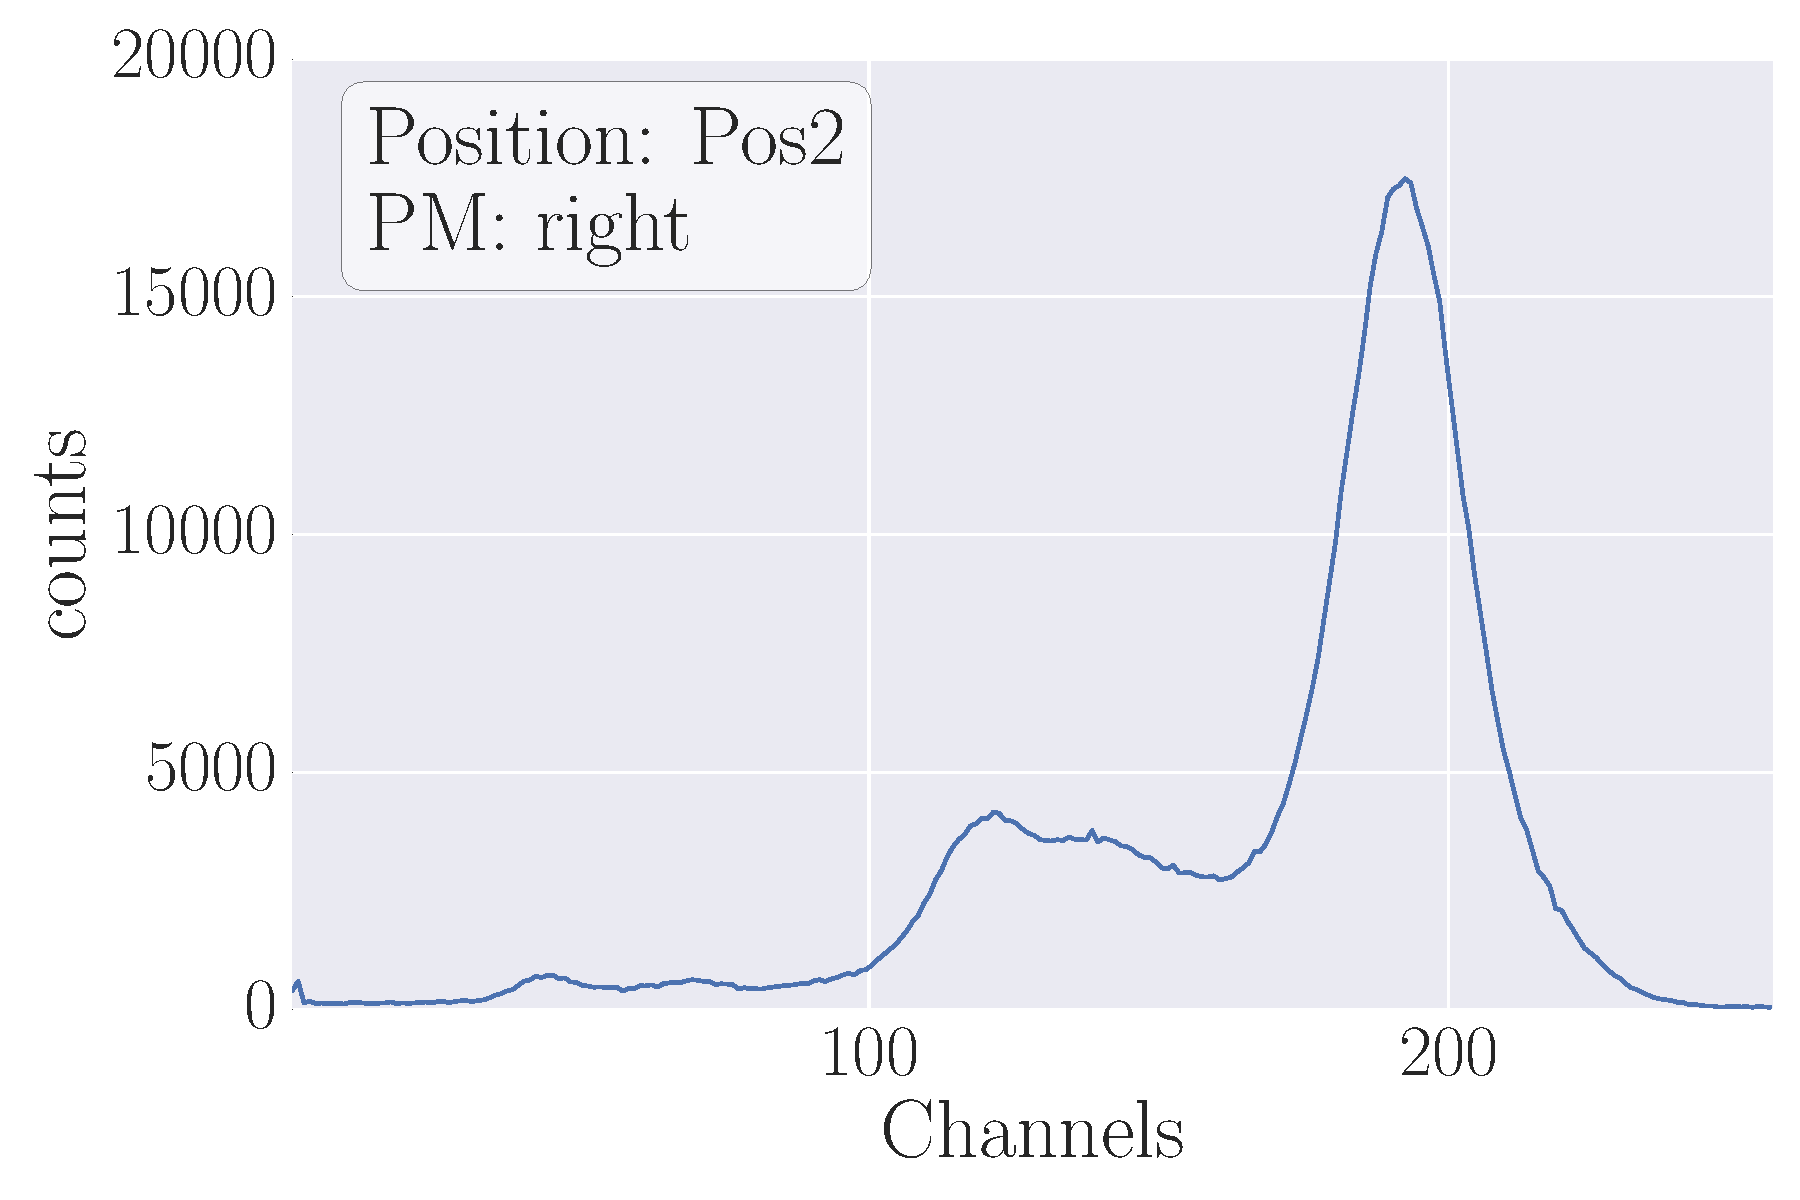
\includegraphics[width=\textwidth]{analysis/figures/plot2_1c}
        \caption{}
    \end{subfigure}
    \begin{subfigure}[b]{\picwidth}
        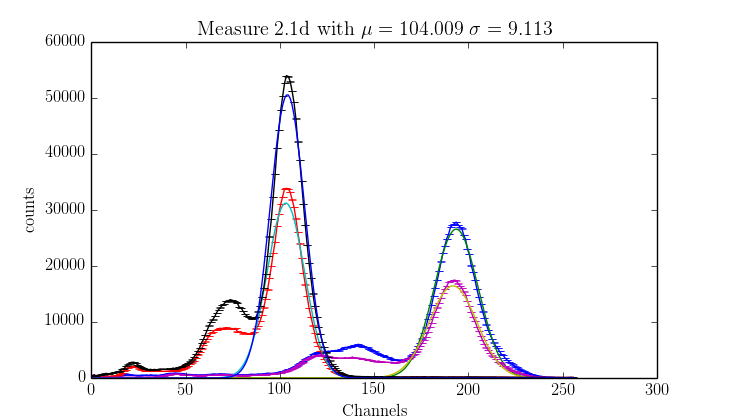
\includegraphics[width=\textwidth]{analysis/figures/plot2_1d}
        \caption{}
    \end{subfigure}
    \begin{subfigure}[b]{\picwidth}
        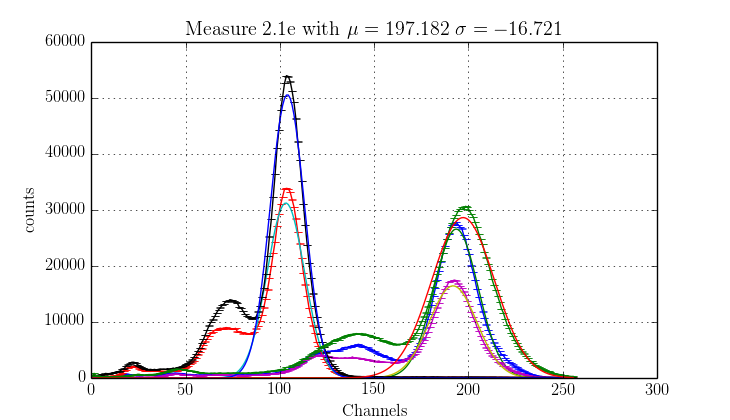
\includegraphics[width=\textwidth]{analysis/figures/plot2_1e}
        \caption{}
    \end{subfigure}
    \caption{
        Histograms of events recorded with the MCA, thus corresponding to the energy 
        spectrum of the probe. Each histogram corresponds to a combination of position 
        of the probe and used detector, as classified in table \ref{tab:config2}
        }
    \label{fig:measure2.1}
\end{figure}

\begin{figure}[htpb]
    \centering
    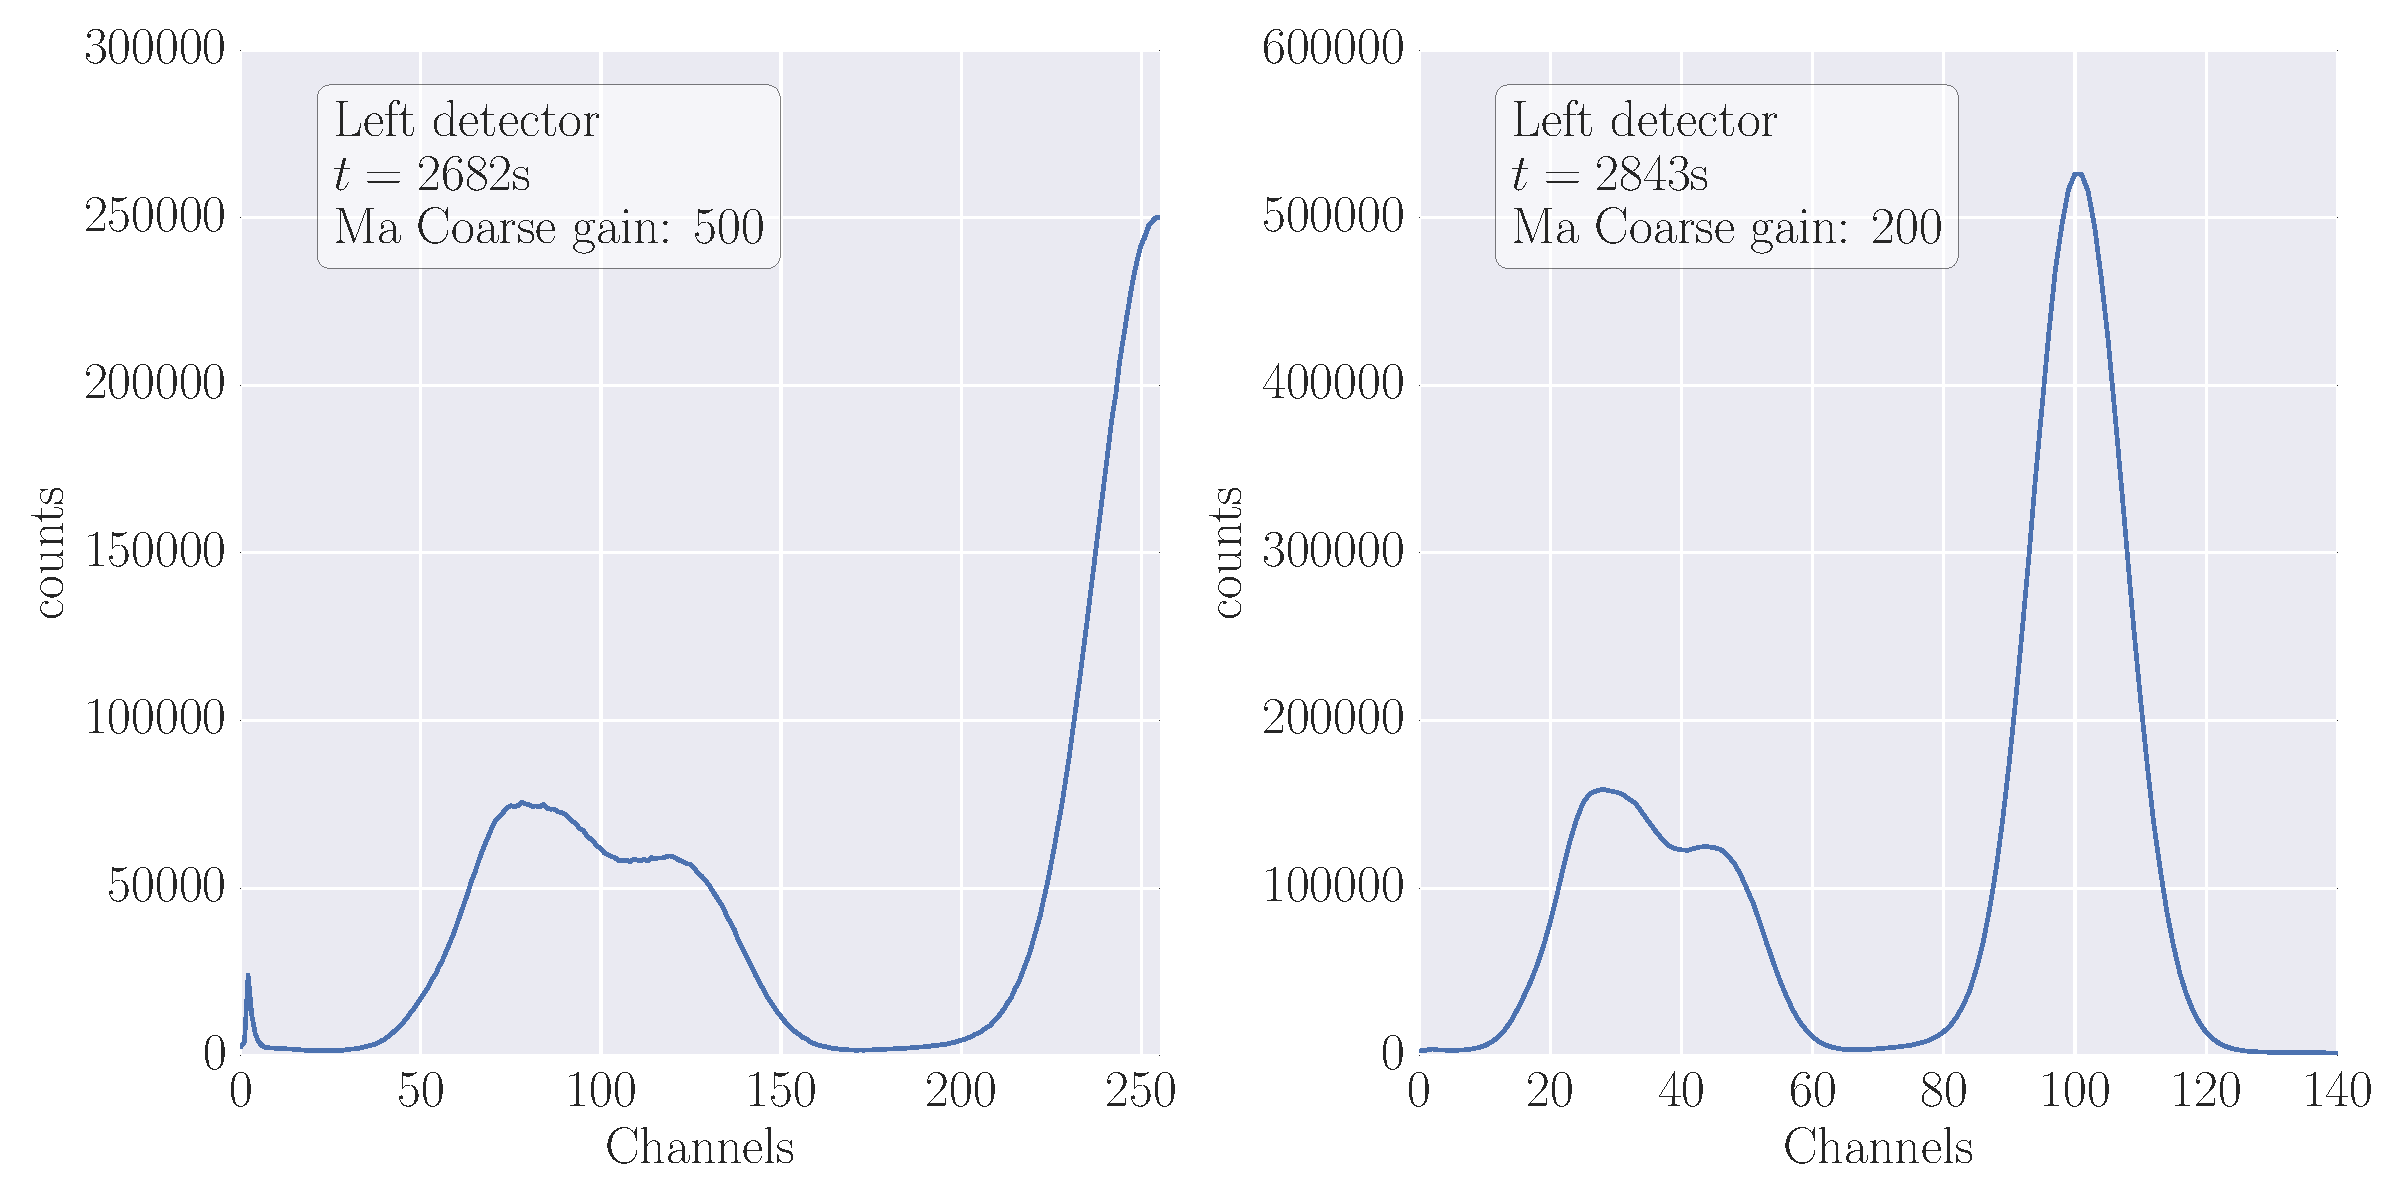
\includegraphics[width=\linewidth]{analysis/figures/plot6_12}
    \caption{$^{241}Am$ energy spectrum}
    \label{fig:plot6_13}
\end{figure}

\begin{figure}[htpb]
    \centering
    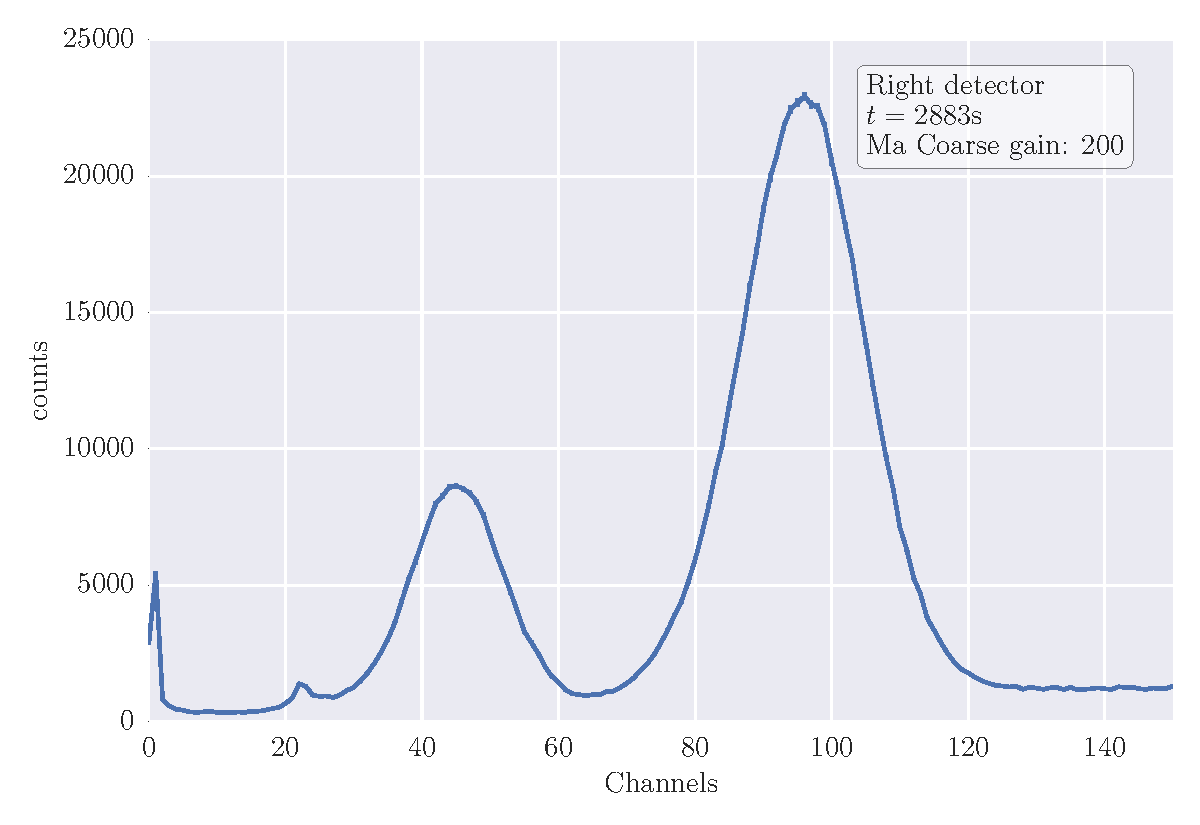
\includegraphics[width=0.8\linewidth]{analysis/figures/plot6_3}
    \caption{$^{241}Am$ energy spectrum}
    \label{fig:plot6_13}
\end{figure}




